\chapter{Lezione 7}
\label{chap:lezione_07} 

\begin{flushright}
\textit{Data: 22/10/2025}
\end{flushright}

\section{Self-Organized Criticality e il Modello Sandpile}

In questa lezione analizziamo la \textit{Self-Organized Criticality} (SOC), un concetto fondamentale per comprendere come i sistemi complessi possano evolvere spontaneamente verso uno stato critico senza la necessità di sintonizzare parametri esterni. Questo approccio è utile per esplorare i metodi di calcolo degli esponenti critici. Il modello di riferimento è il \textbf{Sandpile Model} (o modello della pila di sabbia), introdotto nel 1987 come un "toy model" ispirato alle pile di sabbia reali.

\subsubsection{Dinamica del Modello}
Consideriamo una topologia specifica, in questo caso un reticolo rettangolare bidimensionale (2D). La dinamica è definita dalle seguenti regole:
\begin{enumerate}
    \item \textbf{Iniezione di energia:} Si lascia cadere "energia" (rappresentata da cubi o granelli) sul reticolo.
    \item \textbf{Instabilità e Valanghe:} Quando in un sito si accumulano 4 cubi, il sito diventa instabile. L'instabilità provoca una ridistribuzione dell'energia ai siti vicini.
    \item Se un sito possiede 3 cubi, è definito "instabile" nel senso che l'aggiunta di un solo ulteriore cubo innesca la valanga.
\end{enumerate}

Se si continua a iniettare energia nel sistema, questo raggiungerà asintoticamente uno \textbf{Stato Stazionario}. In questo stato, le valanghe (definite come la sequenza di eventi di ridistribuzione) seguono una distribuzione a legge di potenza (power-law) per dimensioni infinite. Possiamo misurare diverse osservabili fisiche relative alle valanghe:
\begin{itemize}
    \item La dimensione lineare o diametro ($r$).
    \item La dimensione totale ($s$, numero di siti coinvolti o granelli spostati).
    \item La durata temporale ($t$).
\end{itemize}
Sperimentalmente si osserva che le distribuzioni di probabilità di queste grandezze sono tutte leggi di potenza.
In questo contesto, distinguiamo tra:
\begin{itemize}
    \item \textit{Fast modes}: i modi veloci legati alla dinamica delle valanghe.
    \item \textit{Slow modes}: i modi lenti legati all'iniezione di energia dall'esterno.
\end{itemize}

\subsection{Relazioni di Scaling e Esponenti Critici}

Definiamo le distribuzioni di probabilità e le relazioni di scala tra le variabili. Dagli esperimenti e dalle simulazioni emerge che:

\begin{align}
    P(s) &\sim s^{-\tau} \label{eq:Ps} \\
    P(r) &\sim r^{-\lambda} \label{eq:Pr} \\
    P(t) &\sim t^{-\alpha} \label{eq:Pt}
\end{align}

Le variabili stesse sono collegate da relazioni di scala:
\begin{align}
    t &\sim s^x \label{eq:t_s} \\
    t &\sim r^z \label{eq:t_r} \\
    s &\sim r^D \label{eq:s_r}
\end{align}

Dove $z$ è definito come l'\textbf{esponente dinamico}.
Non tutti questi esponenti sono indipendenti. L'obiettivo è calcolare gli esponenti critici derivandoli l'uno dall'altro e risolvendo il modello. Per fare ciò, utilizzeremo il \textbf{Gruppo di Rinormalizzazione nello Spazio Reale}, analizzando come cambia il sistema al variare della scala.

\subsubsection{Derivazione delle Relazioni tra Esponenti}

Cerchiamo di correlare l'esponente $\tau$ con gli esponenti $D$ e $\lambda$.
Consideriamo la conservazione della probabilità tra le distribuzioni di dimensione $s$ e dimensione lineare $r$:
\begin{equation}
    P(s) ds = P(r) dr
\end{equation}
Dalla relazione $s \sim r^D$, differenziando rispetto a $r$ otteniamo:
\begin{equation}
    \frac{ds}{dr} \sim \frac{d}{dr}(r^D) \sim r^{D-1} \implies ds \sim r^{D-1} dr
\end{equation}
Sostituendo le leggi di potenza (\ref{eq:Ps}) e (\ref{eq:Pr}) nell'uguaglianza delle probabilità:
\begin{equation}
    s^{-\tau} ds = r^{-\lambda} dr
\end{equation}
Esprimiamo $s$ in termini di $r$ nel lato sinistro:
\begin{equation}
    (r^D)^{-\tau} \cdot r^{D-1} dr \sim r^{-\lambda} dr
\end{equation}
Semplificando le potenze di $r$:
\begin{equation}
    r^{-D\tau} \cdot r^{D-1} \sim r^{-\lambda} \implies r^{-D\tau + D - 1} \sim r^{-\lambda}
\end{equation}
Uguagliando gli esponenti:
\begin{equation}
    -D\tau + D - 1 = -\lambda
\end{equation}
Moltiplicando per $-1$ e riordinando, otteniamo la prima relazione fondamentale:
\begin{equation}
    \lambda = D(\tau - 1) + 1
\end{equation}

Ora correliamo gli esponenti temporali. Sappiamo che $t \sim s^x$. Possiamo anche scrivere $t \sim r^z$ e, dato che $s \sim r^D$, segue che:
\begin{equation}
    t \sim (r^D)^x = r^{Dx}
\end{equation}
Confrontando con $t \sim r^z$, otteniamo la relazione tra $z$, $D$ e $x$:
\begin{equation}
    z = Dx \implies x = \frac{z}{D}
\end{equation}
Usiamo la conservazione della probabilità tra $s$ e $t$:
\begin{equation}
    P(s) ds = P(t) dt
\end{equation}
Sostituendo le distribuzioni note:
\begin{equation}
    s^{-\tau} ds = t^{-\alpha} dt
\end{equation}
Dalla relazione $t \sim s^x$, differenziando otteniamo $dt \sim x s^{x-1} ds$. Sostituendo:
\begin{equation}
    s^{-\tau} ds \sim t^{-\alpha} (s^{x-1} ds)
\end{equation}
Esprimiamo $t$ in funzione di $s$ ($t \sim s^x$):
\begin{equation}
    s^{-\tau} \sim (s^x)^{-\alpha} \cdot s^{x-1} = s^{-\alpha x} \cdot s^{x-1} = s^{-\alpha x + x - 1}
\end{equation}
Uguagliando gli esponenti di $s$:
\begin{equation}
    -\tau = -x\alpha + x - 1
\end{equation}
Isoliamo $\alpha$:
\begin{equation}
    x\alpha = \tau + x - 1 \implies \alpha = \frac{\tau - 1}{x} + 1
\end{equation}
Sostituendo $x = z/D$:
\begin{equation}
    \alpha = 1 + \frac{D}{z}(\tau - 1)
\end{equation}
Abbiamo quindi un set di esponenti $\tau, z, D, \lambda, \alpha$.
L'analisi dimensionale suggerirebbe che per $d=2$ si abbia $D=2$, ma i sistemi frattali mostrano deviazioni. Se conosciamo $D, \tau, z$, possiamo derivare tutti gli altri.
Valori sperimentali o numerici tipici sono:
\begin{itemize}
    \item $D \simeq 2.75 \pm 0.05$.
    \item In altri casi $D \simeq 3.25 \pm 0.25$.
\end{itemize}
Si tratta di esponenti frattali (non interi). Il nostro obiettivo è trovare un metodo analitico per calcolarli.

\subsection{Procedura di Coarse-Graining}
Applichiamo il metodo del \textit{Coarse-Graining} (granulazione grossolana). Guardiamo il sistema a due scale differenti: la scala $k$ e la scala $k+1$.
L'idea è raggruppare insieme porzioni del sistema ("patches") per formare unità più grandi. Consideriamo un blocco di $2 \times 2$ siti alla scala $k$. Questi 4 siti diventano una singola unità alla scala $k+1$. Vogliamo trovare una dinamica invariante di scala (scale-invariant dynamics).
Si tratta di un processo combinatorio.

Definiamo il vettore delle probabilità alla scala microscopica più bassa ($k=0$):
\begin{equation}
    \vec{P}^{(0)} = (0, 0, 0, 1)
\end{equation}
Le componenti di questo vettore rappresentano la probabilità di scaricare energia su 1, 2, 3 o 4 siti vicini. Alla scala microscopica, in un reticolo quadrato, un sito scarica sempre su tutti e 4 i vicini, quindi $P_4^{(0)} = 1$ e gli altri sono nulli.

Passando alla scala $k$, avremo un vettore generico $\vec{P}^{(k)}$ con norma unitaria $\sum P_i^{(k)} = 1$.
Nel passaggio di coarse-graining alla scala $k+1$, definiamo $\rho^{(k+1)}$ come la densità dei siti critici (density of critical state).
Fisicamente, $\rho$ rappresenta la densità delle pile che stanno per crollare se viene aggiunto un altro granello.

\subsubsection{Equazioni di Rinormalizzazione Autoconsistenti}
Dobbiamo calcolare le probabilità di trasferimento alla scala successiva. Definiamo $W_\alpha$ come la probabilità di avere una configurazione critica su un blocco di dimensione maggiore. Le probabilità per le configurazioni critiche sono date da:
\begin{align}
    W_2 &= 4\rho^2(1-\rho)^2 \\
    W_3 &= 4\rho^3(1-\rho) \\
    W_4 &= \rho^4
\end{align}
Queste rappresentano le probabilità combinatorie che 2, 3 o 4 siti nel blocco siano critici (assumendo indipendenza in campo medio). Nello Stato Stazionario, la quantità di energia che entra deve essere uguale a quella che esce in media. L'energia è costante in media:
\begin{equation}
    \delta E^{(k+1)} = \rho^{(k+1)}
\end{equation}
L'energia trasferita a seguito di una valanga alla scala $k+1$ è proporzionale a $\rho^{(k+1)}$.
L'equazione di bilancio (punto fisso) che lega la densità critica alle probabilità di trasferimento è data da:
\begin{equation}
    \rho^{(k+1)} = \frac{1}{\sum_{n=1}^4 n P_n^{(k+1)}} = \frac{1}{P_1^{(k+1)} + 2P_2^{(k+1)} + 3P_3^{(k+1)} + 4P_4^{(k+1)}}
\end{equation}
Le probabilità $P_n^{(k+1)}$ sono a loro volta determinate da una somma pesata sui $W_\alpha$:
\begin{equation}
    P_n^{(k+1)} = \sum_{\alpha \in \{2,3,4\}} W_\alpha P_n^{(k+1)}(\alpha)
\end{equation}
Dove $P_n^{(k+1)}(\alpha)$ è la probabilità che il super-sito scarichi su $n$ vicini dato che internamente ha $\alpha$ sottositi critici.
Come indicato nelle note, il calcolo esplicito di questi termini coinvolge coefficienti binomiali (es. $\binom{4}{2}$ per scegliere quali siti sono critici).

\subsubsection{Calcolo dell'esponente $\tau$}
Definiamo la \textbf{Stop Probability} $R$ come la probabilità che, a una qualsiasi scala, la valanga si fermi (non propaghi alla scala successiva).
La valanga si ferma se, trasferendo energia su $n$ siti, nessuno di questi è critico. Quindi:
\begin{equation}
    R = P_1^* (1 - \rho^*) + P_2^* (1 - \rho^*)^2 + P_3^* (1 - \rho^*)^3 + P_4^* (1 - \rho^*)^4
\end{equation}
dove l'asterisco indica i valori al punto fisso della rinormalizzazione.

Possiamo collegare $R$ alla distribuzione delle valanghe. La probabilità che una valanga si fermi tra la scala $a(k)$ e la scala $a(k+1)$ è data dall'integrale della distribuzione $P(r)$ in quell'intervallo.
Definiamo la scala minima come $a(k) = a_0 2^k$.
Dalla relazione $P(r) \sim r^{-\lambda}$ e sapendo che $\lambda = 1 + D(\tau-1)$, scriviamo:
\begin{equation}
    P(r) \sim r^{-(1 + D(\tau - 1))}
\end{equation}
La probabilità di arresto $R$ corrisponde all'integrale della distribuzione nell'intervallo di scala considerato:
\begin{equation}
    R \approx \text{Pr}(\text{stop tra } k \text{ e } k+1) = \int_{a(k)}^{a(k+1)} P(r) dr
\end{equation}
Sostituendo la legge di potenza:
\begin{equation}
    R \sim \int_{a(k)}^{a(k+1)} r^{-(1 + D(\tau - 1))} dr
\end{equation}
Risolviamo l'integrale definito tra $a(k)$ e $a(k+1) = 2a(k)$:
\begin{equation}
    R \sim \left[ \frac{r^{-D(\tau-1)}}{-D(\tau-1)} \right]_{a(k)}^{2a(k)} \propto a(k)^{-D(\tau-1)} (1 - 2^{-D(\tau-1)})
\end{equation}
Analizzando il comportamento di scaling e invertendo la relazione per $\tau$, si ottiene la formula finale:
\begin{equation}
    \tau = 1 - \frac{1}{D} \frac{\ln(1 - R^*)}{\ln 2}
\end{equation}
Sostituendo i valori numerici ottenuti dal punto fisso, si trova $\tau \approx 1.253$.
Il valore esatto è $\tau = 5/4 = 1.25$.
Per $D$, gli esperimenti suggeriscono $D \approx 2$.

\subsubsection{Calcolo dell'esponente dinamico $z$}
Vogliamo ora determinare l'esponente dinamico $z$, che lega tempo e spazio ($t \sim r^z$).
Consideriamo la durata media di una valanga alla scala $k$, $\langle t \rangle^{(k)}$.
Nella rinormalizzazione temporale, cerchiamo di capire come scala il tempo tra $k$ e $k+1$.
L'esponente $z$ è dato da:
\begin{equation}
    z = \frac{\ln \langle t \rangle}{\ln 2}
\end{equation}
Dove il fattore 2 al denominatore deriva dal raddoppio della scala spaziale ($a(k+1)/a(k)~=~2$); $\langle t \rangle$ rappresenta il fattore di riscalamento temporale medio derivato dalle equazioni dinamiche del gruppo di rinormalizzazione.

\section{La Scienza delle Reti}
\label{chap:network_science}

La \textit{Network Science} è un campo di studio interdisciplinare che analizza la topologia delle interazioni nei sistemi complessi. A differenza della teoria dei grafi classica, che si occupa di proprietà astratte, la scienza delle reti si concentra sulla struttura e sulla dinamica di reti reali (tecnologiche, sociali, biologiche).

\subsection{Il Problema dei Ponti di Königsberg}
La nascita della teoria dei grafi è convenzionalmente datata 1736, con la soluzione di Eulero al problema dei ponti di Königsberg. La città prussiana presentava 7 ponti che collegavano due isole e le rive del fiume Pregel. Il quesito era: \textit{è possibile ideare un percorso che attraversi ogni ponte esattamente una volta?}

Eulero astrasse il problema trasformando la mappa geografica in un grafo:
\begin{itemize}
    \item \textbf{Nodi:} Le quattro zone di terra ferma.
    \item \textbf{Archi:} I sette ponti.
\end{itemize}
Eulero si concentrò sulla topologia e dimostrò che l'esistenza di tale percorso (oggi chiamato \textbf{cammino euleriano}) dipende esclusivamente dai gradi dei nodi.

\begin{tcolorbox}[colback=colorC!15, colframe=colorC!70!colorB,  title=\textbf{Teorema di Eulero-Hierholzer}]
Una condizione necessaria (e sufficiente per grafi connessi) affinché esista un cammino che attraversa ogni arco una sola volta è che il numero di nodi con grado dispari sia esattamente \textbf{zero} o \textbf{due}.
\end{tcolorbox}
\begin{itemize}
    \item Se non ci sono nodi di grado dispari, il cammino è un \textbf{circuito euleriano} (inizia e finisce nello stesso punto).
    \item Se ci sono due nodi di grado dispari, il cammino deve iniziare in uno di essi e terminare nell'altro.
\end{itemize}
Nel caso di Königsberg, i quattro nodi avevano tutti gradi dispari ed il cammino era impossibile.

\subsection{Classificazione e Tipologie di Reti}
Le reti possono essere categorizzate in base alla natura dei loro nodi e delle interazioni.

\subsubsection{Reti Tecnologiche}
\begin{itemize}
    \item \textbf{Internet:} Rappresenta l'infrastruttura fisica (cavi, router, fibre ottiche). La sua struttura è decentralizzata e gerarchica, composta da \textit{Backbone} (connessioni a lunga distanza ad alta larghezza di banda), \textit{ISP Regionali} e \textit{ISP Locali} che connettono gli utenti finali. 
    \item \textbf{World Wide Web (WWW):} È una rete "logica" di informazioni costruita sopra Internet. I nodi sono le pagine web e gli archi sono i collegamenti ipertestuali (URL).
    \item \textbf{Reti Infrastrutturali:} Esempio rilevante è la rete europea dei gasdotti. 
\end{itemize}


\subsubsection{Reti di Informazione}
\begin{itemize}
    \item \textbf{Wikipedia:} Una rete massiva di collaborazione.
    \item \textbf{Reti di Citazioni:} I nodi sono articoli scientifici e un arco diretto rappresenta una citazione da un articolo all'altro.
\end{itemize}

\subsubsection{Reti Sociali e Social Balance}
Le reti sociali mappano le interazioni tra individui (amicizia, collaborazioni, parentele).
Un esempio storico è la rete delle famiglie fiorentine del XV secolo. L'ascesa dei Medici, pur non essendo la famiglia più ricca, è stata attribuita alla loro posizione topologica strategica nella rete di matrimoni e affari, che ha permesso loro di agire come intermediari tra famiglie rivali disconnesse.

\hfill 

\noindent \textbf{Social Balance:} Le relazioni sociali possono essere positive (amicizia $+1$) o negative (inimicizia $-1$). Consideriamo una triade di nodi collegati $i, j, k$. La triade si dice \textbf{bilanciata} se il prodotto dei segni delle relazioni è positivo:
\begin{equation}
    S_{ij} S_{jk} S_{ki} = 1
\end{equation}
Le configurazioni stabili sono:
\begin{enumerate}
    \item Tre amici ($+, +, +$).
    \item Due nemici e un amico comune ($+, -, -$): "Il nemico del mio nemico è mio amico".
\end{enumerate}
Le configurazioni instabili (sbilanciate con prodotto $-1$) tendono a evolvere dinamicamente verso l'equilibrio.

\hfill 

\noindent \textbf{Small World Effect:} L'esperimento di Milgram (1967) ha introdotto il concetto di "Piccolo Mondo".
A partecipanti casuali nel Midwest USA fu chiesto di far recapitare un pacchetto a un target a Boston, passandolo solo a conoscenti diretti. La lunghezza media delle catene completate era di circa 6 passaggi.

Questo ha dato origine all'espressione "6 gradi di separazione": nonostante le grandi dimensioni della rete sociale, la distanza media tra due nodi qualsiasi è molto piccola.


\subsection{Struttura di un Grafo}
Un grafo $G(v, e)$ è un oggetto matematico composto da:
\begin{itemize}
    \item Un insieme di \textbf{nodi} (o veritici) $v$.
    
    Esempio: $\{a, b, c, d\}$.
    \item Un insieme di \textbf{archi} (o link/edges) $e$, costituiti da coppie di nodi. 
    
    Esempio: $\{(a, b), (a, c), (b, c), (b, d)\}$.
\end{itemize}


\noindent Definiamo le seguenti misure fondamentali:
\begin{itemize}
    \item \textbf{Grado ($k$):} Il numero di archi incidenti su un nodo specifico.
    \item \textbf{Adiacenza:} Due nodi sono adiacenti (distanza = 1) quando sono collegati da un arco.
    \item \textbf{Densità:} È definita come il numero di archi presenti in una rete semplice diviso per il numero massimo di archi possibili.
    \item \textbf{Rete Completa:} Una rete che possiede la massima densità possibile (tutti i nodi sono collegati tra loro).
\end{itemize}

\noindent Per i \textbf{grafi diretti}, il concetto di grado si suddivide in:
\begin{itemize}
    \item \textbf{In-degree ($k_{in}$):} Il numero di archi che il nodo riceve (frecce entranti).
    \item \textbf{Out-degree ($k_{out}$):} Il numero di archi che il nodo invia (frecce uscenti).
\end{itemize}

Il grado totale è la somma: $k = k_{in} + k_{out}$.

\hfill 

\noindent La distanza tra due nodi è definita come il numero minimo di archi necessari per collegarli. Questo percorso minimo è chiamato \textit{shortest path} o \textbf{cammino geodetico}.
Esistono algoritmi specifici per calcolare il cammino geodetico. Nelle reti reali si osserva spesso lo "Small-world effect", ovvero la distanza media tra i nodi è sorprendentemente piccola.

\subsection{Matrice di Adiacenza}
La struttura topologica di una rete è completamente descritta dalla sua \textbf{matrice di adiacenza} $A$. 

\subsubsection{\textcolor{colorA}{Grafi Non Diretti}}
Per un grafo non diretto con $n$ nodi, la matrice di adiacenza $A$ è una matrice quadrata $n \times n$ simmetrica. Gli elementi sono definiti come segue:
\begin{equation}
A_{ij} = 
\begin{cases} 
1 & \text{se esiste un arco tra } i \text{ e } j \\
0 & \text{altrimenti}
\end{cases}
\end{equation}

\noindent Proprietà della matrice:
\begin{itemize}
    \item \textbf{Simmetria:} Poiché il grafo è non diretto, la matrice è simmetrica rispetto alla diagonale principale ($A_{ij} = A_{ji}$).
    \item \textbf{Self-loops:} Se $A_{ii} \neq 0$, significa che esistono collegamenti ricorrenti (cappi) che connettono un nodo a se stesso.
    \item \textbf{Multi-edges:} Se $A_{ii} > 1$, significa che ci sono archi multipli tra la stessa coppia di nodi.
\end{itemize}

\noindent \textbf{{Esempio:}} Consideriamo un grafo con 4 nodi e le connessioni: $(1,2), (1,4), (2,4), (3,4)$.

\hfill

\noindent
\begin{minipage}{0.35\textwidth}
\begin{equation*}
A = 
\begin{pmatrix} 
0 & 1 & 0 & 1 \\ 
1 & 0 & 0 & 1 \\ 
0 & 0 & 0 & 1 \\ 
1 & 1 & 1 & 0 
\end{pmatrix}
\end{equation*}
\end{minipage}%
\hfill
\begin{minipage}{0.55\textwidth}
\centering
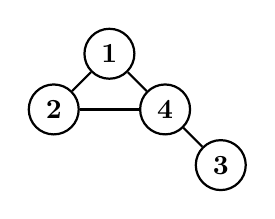
\begin{tikzpicture}[auto, node distance=1cm, thick, scale=0.5,
                    main node/.style={circle,draw,font=\bfseries}]
  \node[main node] (1) {1};
  \node[main node] (2) [below left of=1] {2};
  \node[main node] (4) [below right of=1] {4};
  \node[main node] (3) [below right of=4] {3};

  \path
    (1) edge (2)
    (1) edge (4)
    (2) edge (4)
    (4) edge (3);
\end{tikzpicture}
\end{minipage}



\subsubsection{\textcolor{colorA}{Grafi Pesati Non Diretti}}
La matrice di adiacenza non è necessariamente binaria. È possibile avere una \textbf{forza di interazione} o peso associato a ciascun arco.
La definizione diventa:
\begin{equation}
A_{ij} = 
\begin{cases} 
w_{ij} & \text{peso del collegamento tra } i \text{ e } j \\
0 & \text{se } i \text{ e } j \text{ non sono collegati}
\end{cases}
\end{equation}

\noindent \textbf{Esempio:} 
Consideriamo i seguenti pesi: $w_{1,2}=4$, $w_{1,4}=3.2$, $w_{3,4}=2$, $w_{2,4}=0.5$.

\hfill 

\noindent
\begin{minipage}{0.35\textwidth}
\begin{equation*}
A = 
\begin{pmatrix} 
0 & 4 & 0 & 3.2 \\ 
4 & 0 & 0 & 0.5 \\ 
0 & 0 & 0 & 2 \\ 
3.2 & 0.5 & 2 & 0 
\end{pmatrix}
\end{equation*}
\end{minipage}%
\hfill
\begin{minipage}{0.55\textwidth}
\centering
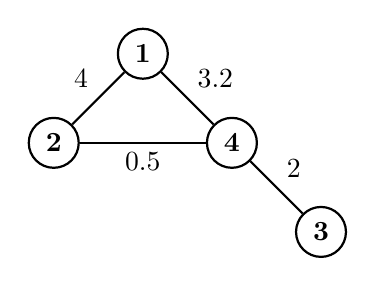
\begin{tikzpicture}[auto, node distance=1.6cm, thick, scale=0.5,
                    main node/.style={circle,draw,font=\bfseries}]
  \node[main node] (1) {1};
  \node[main node] (2) [below left of=1] {2};
  \node[main node] (4) [below right of=1] {4};
  \node[main node] (3) [below right of=4] {3};

  \path
    (1) edge node[above left] {4} (2)
    (1) edge node[above right] {3.2} (4)
    (2) edge node[below] {0.5} (4)
    (4) edge node[above right] {2} (3);
\end{tikzpicture}
\end{minipage}

\hfill \\


\noindent Dato un grafo non diretto con $N$ nodi, il grado $k_i$ del nodo $i$ è definito come il numero di connessioni che esso possiede. In termini di matrice di adiacenza:
\begin{tcolorbox}[colback=yellow!25, colframe=yellow!75!orange, coltitle=black, title=\textbf{Grado di un nodo}]
\begin{equation}
k_i = \sum_{j=1}^N A_{ij}
\end{equation}
\end{tcolorbox}
\noindent Il numero totale di archi $m$ nella rete è legato alla somma dei gradi dalla seguente relazione (Handshake Lemma):
\begin{equation}
\sum_{i=1}^N k_i = \sum_{i=1}^N \sum_{j=1}^N A_{ij} = 2m
\end{equation}
Il fattore 2 deriva dal fatto che ogni arco connette due nodi e viene quindi contato due volte nella sommatoria (una volta per $i$ e una volta per $j$).
Possiamo quindi scrivere:
\begin{tcolorbox}[colback=yellow!25, colframe=yellow!75!orange, coltitle=black, title=\textbf{Numero totale di archi}]
\begin{equation}
m = \frac{1}{2} \sum_{i,j} A_{ij}
\end{equation}
\end{tcolorbox}
\noindent Il \textbf{grado medio} $\langle k \rangle$ è dato da:
\begin{tcolorbox}[colback=yellow!25, colframe=yellow!75!orange, coltitle=black, title=\textbf{Grado medio}]
\begin{equation}
\langle k \rangle = \frac{1}{N} \sum_{i=1}^N k_i = \frac{2m}{N}
\end{equation}
\end{tcolorbox}

\newpage
\subsubsection{\textcolor{colorA}{Grafi Diretti}}
Nei grafi diretti, l'interazione ha una direzione. La matrice di adiacenza $A$ \textbf{non è simmetrica}.
È cruciale definire la convenzione utilizzata, poiché cambia la lettura della matrice. Adottiamo la seguente convenzione (\textbf{Input Convention}):
\begin{equation}
A_{ij} = 
\begin{cases} 
1 & \text{se c'è un link \textbf{da} } j \text{ A } i \quad (j \to i) \\
0 & \text{altrimenti}
\end{cases}
\end{equation}
In altre parole, la riga $i$ raccoglie gli input che il nodo $i$ riceve dagli altri nodi ($j$).

\noindent \textbf{Esempio:} 
Consideriamo archi diretti: $1 \to 2$, $1 \to 3$, $3 \to 2$, $3 \to 4$, $4 \to 3$.

\hfill 

\noindent
\begin{minipage}{0.35\textwidth}
\begin{equation*}
A = 
\begin{pmatrix} 
0 & 0 & 0 & 0 \\ 
1 & 0 & 1 & 0 \\ 
1 & 0 & 0 & 1 \\ 
0 & 0 & 1 & 0 
\end{pmatrix}
\end{equation*}

\end{minipage}%
\hfill
\begin{minipage}{0.55\textwidth}
\centering
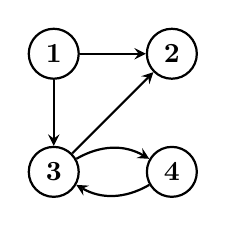
\begin{tikzpicture}[->, >=stealth, auto, node distance=1.5cm, thick, scale=0.5,
                    main node/.style={circle,draw,font=\bfseries}]
  \node[main node] (1) {1};
  \node[main node] (2) [right of=1] {2};
  \node[main node] (3) [below of=1] {3};
  \node[main node] (4) [below of=2] {4};

  \path
    (1) edge (2)
    (1) edge (3)
    (3) edge (2)
    (3) edge[bend left] (4)
    (4) edge[bend left] (3);
\end{tikzpicture}
\end{minipage}

\hfill

\noindent Analisi della matrice:
\begin{itemize}
    \item Riga 1: tutta zeri $\rightarrow$ Il nodo 1 non riceve link da nessuno.
    \item Riga 2: colonne 1 e 3 $\rightarrow$ Il nodo 2 riceve da 1 e da 3.
    \item Riga 3: colonne 1 e 4 $\rightarrow$ Il nodo 3 riceve da 1 e da 4.
    \item Riga 4: colonna 3 $\rightarrow$ Il nodo 4 riceve da 3.
\end{itemize}


È possibile avere processi dinamici su reti fisse (dinamica \textit{sopra} la topologia) oppure reti con archi dipendenti dal tempo (dinamica \textit{della} topologia). Inoltre, si possono avere feedback loops (cicli di retroazione) tra i due processi.

\hfill \\

\noindent Nei grafi diretti, distinguiamo tra grado entrante ($k_{in}$) e grado uscente ($k_{out}$). Utilizzando la convenzione dell'input ($A_{ij}=1 \iff j \to i$):

\begin{itemize}
    \item \textbf{In-degree ($k_i^{in}$):} Somma sulla riga $i$. Rappresenta il numero di archi che arrivano al nodo $i$.
    \begin{tcolorbox}[colback=yellow!25, colframe=yellow!75!orange, coltitle=black, title=\textbf{Grado Entrante}]
    \begin{equation}
    k_i^{in} = \sum_{j=1}^N A_{ij}
    \end{equation}
    \end{tcolorbox}
    
    
    
    \item \textbf{Out-degree ($k_j^{out}$):} Somma sulla colonna $j$. Rappresenta il numero di archi che partono dal nodo $j$.
     \begin{tcolorbox}[colback=yellow!25, colframe=yellow!75!orange, coltitle=black, title=\textbf{Grado Uscente}]
     \begin{equation}
    k_j^{out} = \sum_{i=1}^N A_{ij}
    \end{equation}
    \end{tcolorbox}
\end{itemize}
Per il numero totale di archi $m$, non vi è il doppio conteggio presente nei grafi non diretti, poiché ogni arco ha una direzione univoca. La somma di tutti i gradi entranti deve eguagliare la somma di tutti i gradi uscenti, ed entrambe sono uguali a $m$:
\begin{equation}
m = \sum_{i=1}^N k_i^{in} = \sum_{j=1}^N k_j^{out} = \sum_{i,j} A_{ij}
\end{equation}
Di conseguenza, il grado medio entrante è uguale al grado medio uscente:
\begin{equation}
\langle k_{in} \rangle = \frac{1}{N}\sum_{i=1}^N k_i^{in} = \frac{m}{N}
\end{equation}
\begin{equation}
\langle k_{out} \rangle = \frac{1}{N}\sum_{j=1}^N k_j^{out} = \frac{m}{N}
\end{equation}
Quindi vale sempre:
 \begin{tcolorbox}[colback=yellow!25, colframe=yellow!75!orange, coltitle=black, title=\textbf{Grado Medio}]
     \begin{equation}
    \langle k_{in} \rangle = \langle k_{out} \rangle
    \end{equation}
\end{tcolorbox}

\noindent La \textbf{densità} $\rho$ della rete è il rapporto tra gli archi esistenti e il numero massimo di archi possibili (che è $\binom{N}{2}$):
\begin{tcolorbox}[colback=yellow!25, colframe=yellow!75!orange, coltitle=black, title=\textbf{Densità}]
\begin{equation}
\rho = \frac{m}{N(N-1)/2} = \frac{\langle k \rangle}{N-1}
\end{equation}
\end{tcolorbox}

Analizziamo il comportamento della densità nel limite di reti di grandi dimensioni, ovvero per $n \gg 1$.
In questo regime, possiamo approssimare $n-1 \approx n$. L'espressione della densità si semplifica in:

\begin{equation}
\rho \approx \frac{\langle k \rangle}{n}
\end{equation}
Essendo una probabilità (o frazione di archi esistenti), la densità è sempre limitata nell'intervallo:
\begin{equation}
0 \le \rho \le 1
\end{equation}
A seconda di come il grado medio $\langle k \rangle$ scala al crescere della dimensione della rete $n$, possiamo distinguere diversi regimi:

\begin{itemize}
    \item \textbf{Reti Dense:} Se il grado medio scala linearmente con la dimensione della rete $\langle k \rangle \propto n$, allora il rapporto si stabilizza e la densità rimane costante al crescere di $n$:
    \begin{equation}
    \rho = \text{const}
    \end{equation}

    \item \textbf{Reti Sparse (Comportamento Sub-lineare):} Se il grado medio cresce, ma più lentamente di $n$ (crescita sub-lineare), allora la densità tende asintoticamente a zero:
    \begin{equation}
    \text{Se } \langle k \rangle \text{ cresce sub-linearmente} \implies \rho \to 0
    \end{equation}

    \item \textbf{Reti Estremamente Sparse (Extremely Sparse Networks):} Questo è il caso più comune nelle reti reali di grandi dimensioni. Qui il grado medio è costante e non dipende dalla dimensione della rete $\langle k \rangle = \text{const}$. Di conseguenza, la densità decresce come l'inverso di $n$:
    \begin{equation}
    \langle k \rangle = \text{const} \implies \rho \sim \frac{1}{n} \to 0
    \end{equation}
\end{itemize}


\subsection{Grafi Diretti Aciclici (DAG)}
Un \textbf{DAG} (Directed Acyclic Graph) è un grafo diretto che non contiene cicli chiusi.
Una proprietà fondamentale dei DAG è legata alla struttura della loro matrice di adiacenza.
\begin{tcolorbox}[colback=colorC!15, colframe=colorC!70!colorB,  title=\textbf{Teorema:}]
Per ogni DAG, esiste almeno un'etichettatura (labeling) dei nodi tale che la matrice di adiacenza risulti \textbf{strettamente triangolare superiore}.
\end{tcolorbox}

Questo significa che:
\begin{equation}
A_{ij} = 0 \quad \text{per tutti gli } i \ge j
\end{equation}
In una matrice triangolare superiore, tutti gli elementi sulla diagonale principale e al di sotto di essa sono nulli. Questo implica che non ci sono link che "tornano indietro" rispetto all'ordine stabilito dei nodi.


\noindent
\begin{minipage}{0.35\textwidth}
{Esempio di Matrice \\ Triangolare Superiore:}
\begin{equation*}
A = 
\begin{pmatrix} 
0 & 1 & 1 & 0 & 1 \\ 
0 & 0 & 0 & 0 & 1 \\ 
0 & 0 & 0 & 0 & 1 \\ 
0 & 0 & 0 & 0 & 0 \\ 
0 & 0 & 0 & 0 & 0 
\end{pmatrix}
\end{equation*}
\end{minipage}
\hfill
\begin{minipage}{0.55\textwidth}
\centering
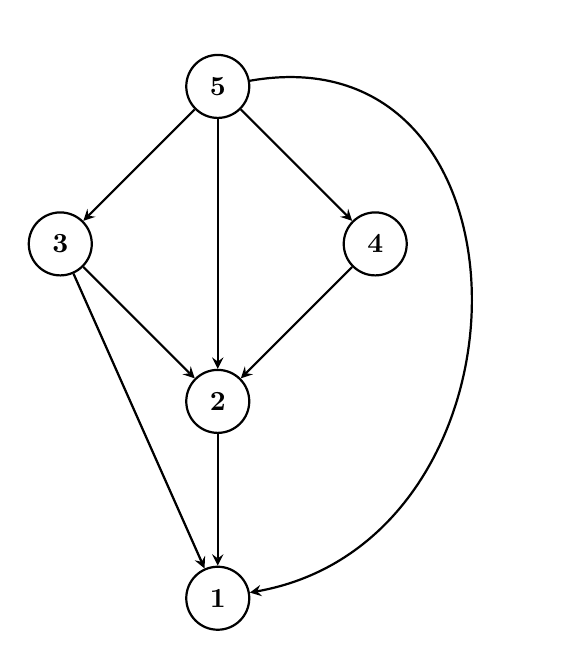
\begin{tikzpicture}[->, >=stealth, auto, node distance=1cm, thick,
                    main node/.style={circle,draw,font=\bfseries,fill=white, minimum size=0.8cm}]

  % Layout gerarchico allargato per evitare sovrapposizioni
  \node[main node] (5) at (0, 4) {5};    % Sorgente
  \node[main node] (3) at (-2, 2) {3};   % Sx
  \node[main node] (4) at (2, 2) {4};    % Dx
  \node[main node] (2) at (0, 0) {2};    % Centro
  \node[main node] (1) at (0, -2.5) {1}; % Pozzo

  \path
    % Da 5 (e)
    (5) edge (3)
    (5) edge (4)
    (5) edge (2) % Passa in mezzo a 3 e 4
    (5) edge[out=10, in=10, looseness=1.5] (1) % Curva larga esterna a sinistra
    
    % Da 4 (d)
    (4) edge (2)
    
    % Da 3 (c)
    (3) edge (2)
    (3) edge (1) % Curva leggera per evitare il nodo 2
    
    % Da 2 (b)
    (2) edge (1);

\end{tikzpicture}
\end{minipage}



\subsection{Reti Bipartite}
Una \textbf{rete bipartita} è un grafo $G=(U,V,E)$ i cui nodi sono divisi in due insiemi disgiunti, $U$ e $V$, tali che ogni arco collega un nodo di $U$ a uno di $V$. Non esistono collegamenti tra nodi appartenenti allo stesso insieme.

Esempi classici includono: Attori e Film ($U$ sono gli attori, $V$ sono i film. Un arco esiste se l'attore recita nel film), Autori e Articoli ($U$ sono gli autori, $V$ sono le pubblicazioni), Entità e Gruppi...


\noindent Poiché la rete connette due classi distinte di oggetti, non si utilizza la classica matrice di adiacenza quadrata, bensì la \textbf{Matrice di Incidenza} $B$.
Se abbiamo $g$ gruppi e $n$ entità, la matrice $B$ avrà dimensione $g \times n$.
La definizione formale è:
\begin{equation}
B_{ij} = 
\begin{cases} 
1 & \text{se l'entità } j \text{ appartiene al gruppo } i \\
0 & \text{altrimenti}
\end{cases}
\end{equation}
\textbf{Rappresentazione Grafica:}
Di seguito è riportato un esempio di rete bipartita con la relativa matrice di incidenza.

\vspace{0.5cm}
\noindent
\begin{minipage}{0.35\textwidth}
\begin{equation*}
B = 
\begin{pmatrix} 
1 & 0 & 1 & 0 & 0 \\ 
0 & 0 & 1 & 0 & 0 \\ 
0 & 1 & 0 & 1 & 0 \\ 
1 & 0 & 0 & 1 & 1 
\end{pmatrix}
\end{equation*}
\end{minipage}%
\hfill
\begin{minipage}{0.55\textwidth}
\centering
\begin{tikzpicture}[thick,
    group node/.style={rectangle,draw,fill=colorC,minimum size=8mm,font=\small\bfseries, text=white,},
    entity node/.style={circle,draw,fill=colorE,minimum size=8mm,font=\small\bfseries}, text=white,]
    
    % Gruppi a sinistra
    \node[group node] (g1) at (0,3) {G1};
    \node[group node] (g2) at (0,2) {G2};
    \node[group node] (g3) at (0,1) {G3};
    \node[group node] (g4) at (0,0) {G4};
    
    % Entità a destra
    \node[entity node] (e1) at (3,3.2) {E1};
    \node[entity node] (e2) at (3,2.4) {E2};
    \node[entity node] (e3) at (3,1.6) {E3};
    \node[entity node] (e4) at (3,0.8) {E4};
    \node[entity node] (e5) at (3,0) {E5};

    % Archi basati sulla matrice B
    \draw (g1) -- (e1);
    \draw (g1) -- (e3);
    \draw (g2) -- (e3);
    \draw (g3) -- (e2);
    \draw (g3) -- (e4);
    \draw (g4) -- (e1);
    \draw (g4) -- (e4);
    \draw (g4) -- (e5);
\end{tikzpicture}
\end{minipage}

\subsubsection{Proiezioni One-Mode}
Spesso si è interessati alle relazioni dirette tra nodi dello stesso tipo (es. "quali attori hanno recitato insieme?"). Per ottenere queste informazioni, si effettua una proiezione della rete bipartita su uno dei due insiemi.

\begin{enumerate}
    \item \textbf{Proiezione Entità-Entità:}
Questa proiezione crea una rete composta solo dalle $n$ entità. Due entità sono collegate se condividono almeno un gruppo.
Matematicamente, si ottiene moltiplicando la trasposta di $B$ per $B$ stessa:
\begin{equation}
P = B^T B
\end{equation}
$P$ è una matrice quadrata $n \times n$ simmetrica. L'elemento generico $P_{ij}$ è dato da:
\begin{equation}
P_{ij} = \sum_{k=1}^g (B^T)_{ik} B_{kj} = \sum_{k=1}^g B_{ki} B_{kj}
\end{equation}
L'interpretazione fisica dei termini è la seguente:
\begin{itemize}
    \item \textbf{Elementi diagonali ($P_{ii}$):} Rappresentano il numero di gruppi a cui partecipa l'entità $i$.
    \item \textbf{Elementi fuori diagonale ($P_{ij}$ con $i \neq j$):} Rappresentano il numero di gruppi che le entità $i$ e $j$ condividono.
\end{itemize}
Per ottenere la matrice di adiacenza classica (binaria o pesata senza self-loops), si impone solitamente $A_{ii} = 0$.
\item \textbf{Proiezione Gruppo-Gruppo:}
Analogamente, possiamo proiettare sui gruppi per vedere quali gruppi condividono entità.
La matrice risultante $P'$ è quadrata di dimensione $g \times g$:
\begin{equation}
P' = B B^T
\end{equation}
L'elemento generico è:
\begin{equation}
P'_{ij} = \sum_{k=1}^n B_{ik} (B^T)_{kj} = \sum_{k=1}^n B_{ik} B_{jk}
\end{equation}
Qui, $P'_{ij}$ indica quante entità sono presenti contemporaneamente sia nel gruppo $i$ che nel gruppo $j$.
\end{enumerate}




\subsection{Alberi}
Un \textbf{albero} è una tipologia fondamentale di grafo. Si definisce albero un grafo connesso e non diretto che non contiene cicli (loops).
\begin{enumerate}
    \item In un albero esiste \textbf{uno e un solo cammino} che collega qualsiasi coppia di vertici.
    \item Un albero con $N$ vertici possiede esattamente $N-1$ archi.
    \item Se si aggiunge un arco a un albero, si crea necessariamente un ciclo.
    \item Se si rimuove un qualsiasi arco da un albero, il grafo diventa sconnesso.
\end{enumerate}

\begin{center}
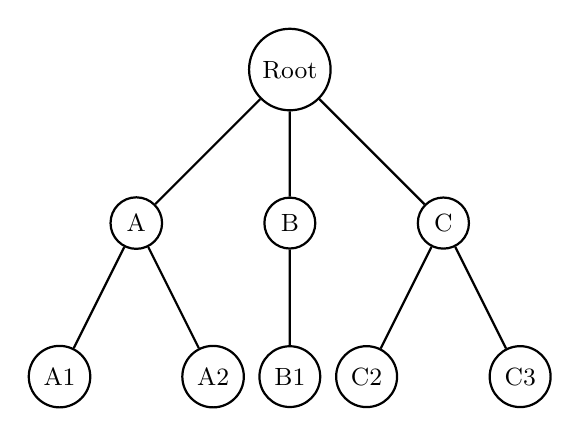
\begin{tikzpicture}[thick, scale=1.3, every node/.style={circle,draw,fill=white,font=\small}]
  \node (root) at (0,0) {Root}
    child {node {A}
      child {node {A1}}
      child {node {A2}}
    }
    child {node {B}
      child {node {B1}}
    }
    child {node {C}
      child {node {C2}}
      child {node {C3}}
    };
\end{tikzpicture}
\end{center}
